\documentclass{tufte-handout}

\title{Notes on SwAV\thanks{Caron, Mathilde, et al. "Unsupervised learning of visual features by contrasting cluster assignments." arXiv preprint arXiv:2006.09882 (2020).}}

\author[The Tufte-LaTeX Developers]{Seri Lee}

%\date{28 March 2010} % without \date command, current date is supplied

%\geometry{showframe} % display margins for debugging page layout

\usepackage{graphicx} % allow embedded images
  \setkeys{Gin}{width=\linewidth,totalheight=\textheight,keepaspectratio}
  \graphicspath{{./images/}} % set of paths to search for images
\usepackage{amsmath}  % extended mathematics
\usepackage{booktabs} % book-quality tables
\usepackage{units}    % non-stacked fractions and better unit spacing
\usepackage{multicol} % multiple column layout facilities
\usepackage{lipsum}   % filler text
\usepackage{fancyvrb} % extended verbatim environments
  \fvset{fontsize=\normalsize}% default font size for fancy-verbatim environments
% \usepackage{cite}
\usepackage{amsmath, amssymb, amsfonts}
\usepackage[ruled, vlined]{algorithm2e}
\usepackage{geometry}
\usepackage[utf8]{inputenc}
\usepackage{pgfplots}
\usepackage{textcomp}
\usepackage{xcolor}
\usepackage{verbatim}
\usepackage{tikz}

% \pgfplotsset{width=10cm, compat=1.9}
% Standardize command font styles and environments
\newcommand{\doccmd}[1]{\texttt{\textbackslash#1}}% command name -- adds backslash automatically
\newcommand{\docopt}[1]{\ensuremath{\langle}\textrm{\textit{#1}}\ensuremath{\rangle}}% optional command argument
\newcommand{\docarg}[1]{\textrm{\textit{#1}}}% (required) command argument
\newcommand{\docenv}[1]{\textsf{#1}}% environment name
\newcommand{\docpkg}[1]{\texttt{#1}}% package name
\newcommand{\doccls}[1]{\texttt{#1}}% document class name
\newcommand{\docclsopt}[1]{\texttt{#1}}% document class option name
\newenvironment{docspec}{\begin{quote}\noindent}{\end{quote}}% command specification environment

\begin{document}

\maketitle% this prints the handout title, author, and date

\begin{abstract}
Unsupervised image representations have significantly reduced the gap with supervised pretraining, notably with the recent achievements of contrastive learning methods.
These contrastive methods typically work online and rely on a large number of explicit pairwise feature comparisons, which is computationally challenging.
In the paper mentioned above, they propose an online algorithm, SwAV, that takes advantage of contrastive methods without requiring to compute pairwise comparisons.

Specifically, our method simultaneously clusters the data while enforcing consistency between cluster assignments produced for different augmentations (or ``views'') of the same image,
instead of computing features directly as in contrastive learning.

Simply out, we use a ``swapped'' prediction mechanism where we predict the code of a view from the representation of another view.

Our method can be trained with large and small batches and scale to unlimited amounts of data.
Compared to previous method, our method is more memory efficient since it does not require a large memory bank or a special momentum network.

In addition, we also propose a new data augmentation stratey, $multi-crop$, that uses a mix of views with different resolutions in place of two full-resolution views, without increasing the memory or compute requirements.

We validate our findings by achieving 75.3\% top-1 accuracy on ImageNet with ResNet-50, as well as surpassing supervised pretraining on all the considered transfer tasks.
\end{abstract}

  \begin{table}[ht]
    \centering
    \fontfamily{ppl}\selectfont
    \begin{tabular}{cccc}
      \toprule
      Method & Architecture & Parameter & top-1 accuracy \\
      \midrule
      MoCo & ResNet50 & 24 & 60.6 \\
      PIRL & ResNet50 & 24 & 63.6 \\
      SIMCLR & ResNet50 & 24 & 70.0 \\
      SwAV & ResNet50 & 24 & 75.3 \\
      \bottomrule
    \end{tabular}
    \caption{\textbf{Linear classification on ImageNet}. Top-1 accuracy for linear models trained on frozen features from different self-supervised methods.}
    \label{tab:normaltab}
    %\zsavepos{pos:normaltab}
  \end{table}
%\printclassoptions

\section{Introduction}\label{sec:introductions}
\newthought{Many recent state-of-the-art methods} build upon the instance discrimination task that considers each image of the dataset (``instance'')
and its transformations as a separate class.
This task yields representations that are able to discriminate between different images, while achieving some invariance to image transformations.
Recent self-supervised methods that use instance discrimination rely on a combination of two elements: (1) a contrastive loss and (2) a set of image transformations.

The contrastive loss removes the notion of instance classes by direcly mapping image features while the image transformations define the invariances encoded in the features.
Both elements are essential to the quality of the resulting network. 

\begin{marginfigure}
  \begin{center}
  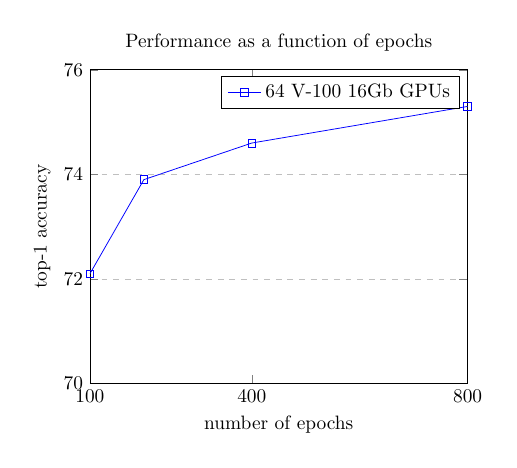
\begin{tikzpicture}[scale=0.7]
    \begin{axis}[
        title={Performance as a function of epochs},
        xlabel={number of epochs},
        ylabel={top-1 accuracy},
        xmin=100, xmax=800,
        ymin=70, ymax=76,
        xtick={100, 400, 800},
        ytick={70, 72, 74, 76},
        ymajorgrids=true,
        grid style=dashed,
    ]
    
    \addplot[
        color=blue,
        mark=square,
        ]
        coordinates {
        (100, 72.1)(200, 73.9)(400, 74.6)(800, 75.3)
        };
        \legend{64 V-100 16Gb GPUs}
        
    \end{axis}
    \end{tikzpicture}
  \end{center}
    \caption{\textbf{Performance as a function of epochs}.Comparing SwAV models trained with different number of epochs and reporting their running time.}
  \label{fig:marginfig}
  \end{marginfigure}

The contrastive loss explicitly compares pairs of image representations to push away representations from different images while pulling together those transformations, or views, of the same image.

Since computing all the pairwise comparisons on a large dataset is not practical, most implementations approximate the loss by reducing the number of comparisons to random subsets of images during training.
An alternative to approximate the loss is to approximate the task-that is to relax the instance discrimination problem.
For example, clustering-based methods discriminate between groups of images with similar features instead of individual images.

The objective in clustering is tractable, but it does not scale well with the dataset as it requires a pass over the entire dataset to form image ``codes'' (\textit{i.e.}, cluster assignments) that are used as targets during training.
In this work, we use a different paradigm and propose to compute the codes online while enforcing consistency between codes obtained from views of the same image.

Comparing cluster assignments allows to contrast different image views while not relying on explicit pairwise feature comparisons.
Specifically, we propose a simple ``swapped'' prediction problem where we predict the code of a view from the representation of another view.

We learn features by Swapping Assignments between multiples Views of the Same Image (SwAV). The features and codes are learned online, allowing our method to scale to potentially unlimited amounts of data.

\begin{figure}
  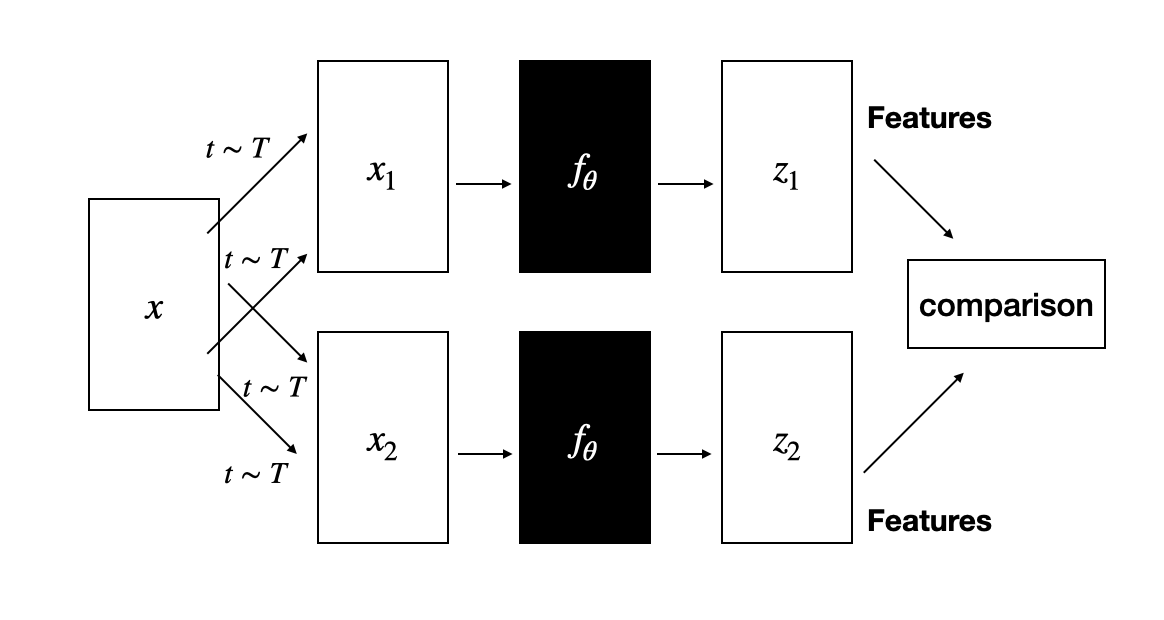
\includegraphics[scale=5]{instance}
%  \checkparity This is an \pageparity\ page.%
  \caption{Contrastive instance learning.
  \emph{the features from different transformations of the same images are compared directly to each other.}}
  \label{fig:textfig}
  %\zsavepos{pos:textfig}
  \setfloatalignment{b}
\end{figure}

\begin{figure}
  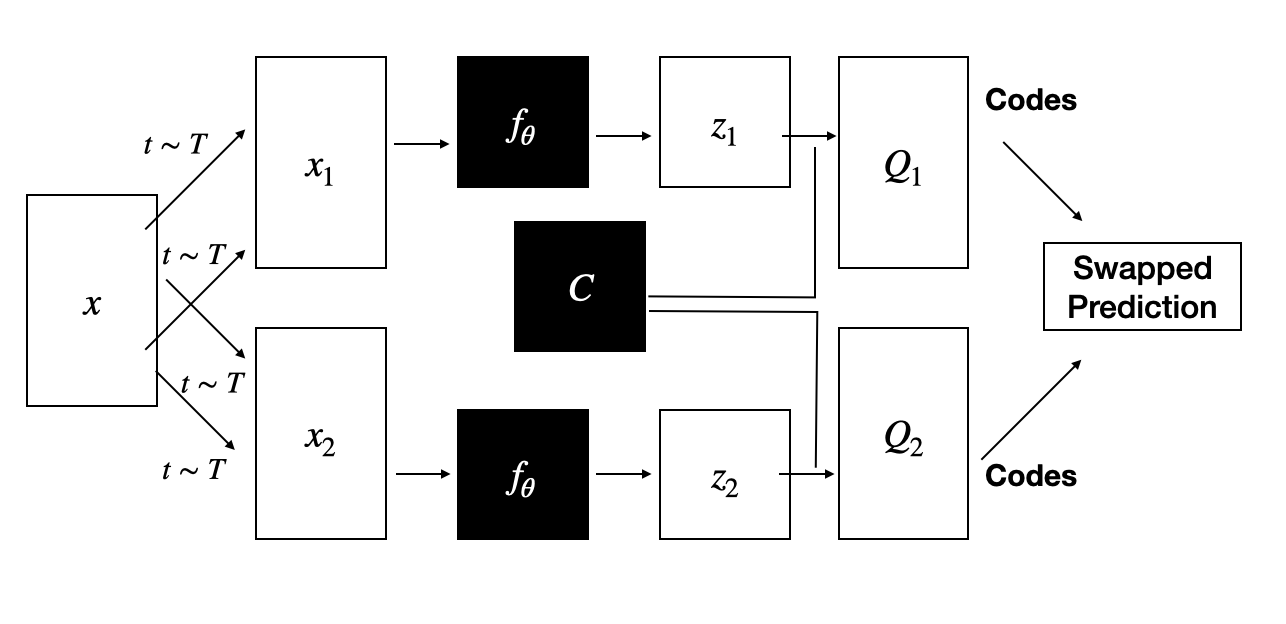
\includegraphics[scale=5]{swav}
%  \checkparity This is an \pageparity\ page.%
  \caption{SwAV.
  \emph{We first obtain ``codes'' by assigning features to prototype vectors. Then solve a ``swapped'' prediction problem wherein the codes obtained from one data augmented view are predicted using the other view.
  Prototype vectors are learned along with the ConvNet parameters by backpropagation.}}
  \label{fig:textfig}
  %\zsavepos{pos:textfig}
  \setfloatalignment{b}
\end{figure}

Besides our online clustering-based method, we also propose an improvement to the image transformations.
Most contrastive methods compare one pair of transformations per image, even though there is evidence that comparing more views during training improves the resulting model.
In this work, we propose $multi-crop$ that uses smaller-sized images to increase the number of views while not increasing the memory or computational requirements during training.
We also observe that mapping small parts of a scene to more global views significantly boosts the performance.

Directly working with downsized images introduces a bias in the features, which can be avoided by using a mix of different sizes.
Our strategy is simple, yet effective, and can be applied to many self-supervised methods with consistent gain in performance.

They validate their contributions by evaluating their protocol on several standard self-supervised benchmarks.
In particular, on the ImageNet linear evaluation protocol, they reach 75.3\% top-1 accuracy with a standard ResNet-50, and 78.5\% with a wider model. 
% \footnote[]{} \marginnote{} \sidenote[]{}
\subsection{Method}\label{sec:method}
Our goal is to learn visual features in an online fashion without supervision. 
To that effect, we propose an online clustering-based self-supervised method.
Typical clustering-based methods are offline in the sense that they alternate between a cluster assignment step where images features of the entire dataset are clustered, 
and a training step where the cluster assignments, \textit{i.e.} ``codes'' are predicted for different image views.
Unfortunately, these methods are not suitable for online learning as they require multiple passes over the dataset to compute the image features necessary for clustering.

In this section, we describe an alternative where we enforce consistency between codes from different augmentations of the same image.
This solution is inspired by contrastive instance learning as we do not consider code as target, but only enforce consistency mapping between views of the same image. \sidenote{This method can be interpreted as a way of contrasting between multiple image views by comparing their cluster asignments instead of their features.}

More precisely, we compute a code from an augmented version of the image and predict this code from other augmented versions of the same image.
Given two image features $z_t$ and $z_s$ from two different augmentations of the same image, we compute their codes $q_t$ and $q_s$ by matching these features to a set of $K$ prototypes ${c_1, \ldots, c_K}$.
We then setup a ``swapped'' prediction problem with the following loss function:
\begin{equation}
  L(z_t, z_s) = l(z_t, q_s) + l(z_s, q_t)
\end{equation}
where the function $l(z,q)$ measures the fit between features $z$ and code $q$, as detailed later. \sidenote{\textbf{Intuitively, this method compares the features $z_t$ and $z_s$ using the intermediate codes $q_t$ and $q_s$.
If these two features capture the same information, it should be possible to predict the code from other feature.}
\textit{A similar comparison appears in contrastive learning where features are compared directly.}}

\subsection{Online clustering}
Each image $x_n$ is transformed into an augmented view $x_{nt}$ by applying a transformation $t$ sampled from the set $T$ of image transformations.
The augmented view is mapped to a vector representation by applying a non-linear mapping $f_\theta$ to $x_{nt}$. 
The feature is then projected to the unit sphere, \textit{i.e.}, $z_{nt} = f_\theta(x_{nt}) / \left\lVert f_\theta(x_{nt}) \right\rVert_{2}$.
We then compute a code $q_{nt}$ from this feature by mapping $z_{nt}$ to a set of $K$ trainable prototypes vectors, ${c_1,\ldots, c_K}$. 
We denote by $C$ the matrix whose columns are the $c_1, \ldots, c_k$. 

\textbf{Swapped prediction problem}
The loss function in Eq.(1) has two terms that setup the ``swapped'' prediction problem of predicting the code $q_t$ from the feature $z_s$, and $q_s$ from $z_t$.
Each term represents the cross entropy loss between the code and the probability obtained by taking a softmax of the dot products of the $z_i$, and all prototypes in $C$, \textit{i.e.},
\begin{equation}
  l(z_t, q_s) = - \sum_{k}q_s^{(k)}\log p_t^{(k)}
\end{equation}
, where
\begin{equation}
  p_t^{(k)} = \frac{exp(\frac{1}{\tau}z_t^\top c_k)}{\sum_{k'}exp(\frac{1}{\tau}z_t^\top c_{k'})}
\end{equation}
where $\tau$ is a temperature parameter. Taking this loss over all the images and pairs of data augmentations leads to the following loss function for swapped prediction problem:
\begin{equation}
  -\frac{1}{N}\sum_{n=1}^N \sum_{t \sim T}[\frac{1}{\tau}z_{ns}^\top C q_{nt} + \frac{1}{\tau}z_{ns}^\top C q_{nt}  -\log\sum_{k=1}^{K}exp(\frac{z_{nt}^\top c_k}{\tau}) -\log\sum_{k=1}^{K}exp(\frac{z_{ns}^\top c_k}{\tau})]
 \end{equation}
This loss function is jointly minimized with respect to the prototypes $C$ and the parameters $\theta$ of the image encoder $f_\theta$ used to produce the features $(z_{nt})_{n,t}$.

\textbf{Computing codes online} In order to make our method online, we compute the codes using only the image features within a batch. 
\sidenote{Intuitively, as the prototypes $C$ are used across different batches, SwAV clusters multiple instances to the prototypes.}
We compute codes using the prototypes $C$ such that all examples in a batch are equally partitioned by the prototypes.

This equipartition constraint ensures that the codes for different images in a batch are distinct, thus preventing the trivial solution where every image has the same code.
Given $B$ feature vectors $Z = [z_1, \ldots, z_B]$, we are interested in mapping them to the prototypes $C = [c_1, \ldots, c_K]$. 
We denote this mapping or codes by $Q = [q_1, \ldots, q_B]$, and optimize $Q$ to maximize the similarity between the features and the prototypes, \textit{i.e.},
\begin{equation}
  \max_{Q \in \mathcal{Q} }Tr(Q^\top C^\top Z) + \varepsilon H(Q)
\end{equation}
where $H$ is the entropy function, $H(Q) = -\sum_{ij}Q_{ij}\log Q_{ij}$ and $\varepsilon$ is a parameter that controls the smoothness of the mapping.
\sidenote{We observe that a strong entropy regularization (\textit{i.e.} using a high $\varepsilon$) generally leads to a trivial solution where all samples collapse into an unique representation and are all assigned uniformly to all prototypes.}
In practice, we keep $\varepsilon$ low. Asano et al. enforce an equal partition by constraining the matrix $Q$ to belong to the transportation polytope. 
They work on the full dataset, and we propose to adapt their solution to work on minibatches by restricting the transportation polytope to the minibatch:
\begin{equation}
  \mathcal{Q} = \{ Q \in \mathbb{R}^{K \times B}_{+} | Q1_B = \frac{1}{K}1_K, Q^{\top}1_K = \frac{1}{B}1_B\}
\end{equation}
where $1_K$ denotes the vector of ones in dimensions $K$. These constraints enforce that on average each prototype is selected at least $\frac{B}{K}$ times in the batch.

Once a continuous solution to $Q^{*}$ to Prob.(5) is found, a discrete code can be obtained by using a rounding procedure.
Empirically, we found that discrete codes work well when computing codes in an offline manner on the full datasets as in Asano et al. 
However, in the online setting where we use only minibatches, using the discrete codes performs worse than using the continuous codes.
\sidenote{An explanation is that the rounding needed to obtain discrete codes is a more aggressive optimization step than gradient updates. While it makes the model converge rapidly, it leads to a worse solution.}
We preserve the soft code $Q^{*}$ instead of rounding it. These soft codes $Q^{*}$ are the solution of Prob.(5) over the set $mathcal{Q}$ and takes the form of a normalized exponential matrix:
\begin{equation}
  Q^{*} = Diag(u)exp(\frac{C^\top Z}{\varepsilon})Diag(v)
\end{equation}
where $u$ and $v$ are renormalization vectors in $\mathbb{R}^K$ and $\mathbb{R}^B$ respectively.
The renormalization vectors are computed using a small number of matrix multiplications using the iterative Sinkhorn-Knopp algorithm.
In practice, we observe that using only three iterations is fast and sufficient to obtain good performance.
Indeed, this algorithm can be efficiently implemented on GPU, and the alignment of 4K features to 3K codes takes 35ms in their experiment.

\textbf{Working with small batches} When the number $B$ of batch features is too small compared to the number of prototypes $K$, it is impossible to equally partition the batch into the $K$ prototypes.
When working with small batches, we use features from the previous batches to augment the size of $Z$ in Prob.(5). 
Then, we only use the codes of the batch features in our training loss. \sidenote{In practice, they store around 3K features in teh same range as the number of code vectors}.
This means that we only keep features from the last 15 batches with a batch size of 256, while contrastive methods typically need to store the last 65K instances obtained from the last 250 batches.

\subsection{$Multi-crop$: Augmenting views with smaller images}
As noted in prior works, comparing random crops of an image plays a central role by capturing information in terms of relations between parts of a scene or an object.
unfortunately, increasing the number of crops or ``views'' quadratically increases the memory and compute requirements. 

We propose $multi-crop$ strategy where we use two standard resolution crops and sample $V$ additional low resolution crops that cover only small parts of the image.
Using low resolution images ensures only a small increase in the compute cost.
Specifically, we generalize the loss of Eq.(1):
\begin{equation}
  L(z_{t_1}, z_{t_2}, \ldots, z_{t_{V+2}}) = \sum_{i \in \{1,2\}} \sum_{v=1}^{V+2} 1_{v \neq i} l(z_{t_v}, q_{t_i})
\end{equation}
Note that we compute codes using only the full resolution crops. Indeed, computing codes for all crops increases the computational time and we observe in practice that it also alters the transfer performance of the resulting network. 
An explanation is that using only partial information (small crops cover only small area of images) degrades the assignment quality.
\section{Main Results}

\section{Ablation Study}
\section{Discussion}




\bibliography{sample-handout}
\bibliographystyle{plainnat}



\end{document}
